    \documentclass{article}
    \usepackage{fancyhdr, amsmath, amsthm, amssymb, mathtools, lastpage, hyperref, enumerate, graphicx, setspace, upgreek}
    \usepackage[margin=1in, top=0.8in,bottom=0.8in]{geometry}
    \usepackage{subcaption}
    \newcommand{\scinot}[2]{#1\times10^{#2}}
    \newcommand{\bra}[1]{\left<#1\right|}
    \newcommand{\ket}[1]{\left|#1\right>}
    \newcommand{\dotp}[2]{\left<#1\,\middle|\,#2\right>}
    \newcommand{\rd}[2]{\frac{\mathrm{d}#1}{\mathrm{d}#2}}
    \newcommand{\pd}[2]{\frac{\partial#1}{\partial#2}}
    \newcommand{\rtd}[2]{\frac{\mathrm{d}^2#1}{\mathrm{d}#2^2}}
    \newcommand{\ptd}[2]{\frac{\partial^2 #1}{\partial#2^2}}
    \newcommand{\norm}[1]{\left|\left|#1\right|\right|}
    \newcommand{\abs}[1]{\left|#1\right|}
    \newcommand{\pvec}[1]{\vec{#1}^{\,\prime}}
    \newcommand{\tensor}[1]{\overleftrightarrow{#1}}
    \let\Re\undefined
    \let\Im\undefined
    \newcommand{\ang}[0]{\text{\AA}}
    \newcommand{\mum}[0]{\upmu \mathrm{m}}
    \DeclareMathOperator{\Re}{Re}
    \DeclareMathOperator{\Tr}{Tr}
    \DeclareMathOperator{\Im}{Im}
    \DeclareMathOperator{\E}{E}
    \DeclareMathOperator{\Var}{Var}
    \newcommand{\expvalue}[1]{\left<#1\right>}
    \usepackage[labelfont=bf, font=scriptsize]{caption}\usepackage{tikz}
    \usepackage[font=scriptsize]{subcaption}
    \everymath{\displaystyle}

\begin{document}
\title{Ph20.2 - Introduction to Numerical Techniques:\\ Numerical Integration}
\author{Cassidy Yang}
\maketitle
\pagestyle{fancy}
\rhead{Cassidy Yang}
\cfoot{Page \thepage \hspace{1pt} of \pageref{LastPage}}

\section{The Assignment}

The corresponding Python code is attached in a separate document.

\begin{enumerate}
	\item Derive extended Simpson's formula.
	
	By elementary definite integration and also an extension of Eq. (4) in the assignment notes, we get
	\begin{equation}
		I = f(a)H + f'(a) \frac{H^2}{2!} + f''(a) \frac{H^3}{3!} + f^{(3)}(a) \frac{H^4}{4!} + f^{(4)}(\eta) \frac{H^5}{5!} + ...   \hspace{2pt} \text{with} \hspace{2pt} \eta \in [a, b].
	\end{equation}		
	
	We can can use \textit{Simpson's rule} from Eq. (8) in the assignment notes and reproduced below where $c = \frac{(a+b)}{2}$
	
	\begin{equation}
		I \simeq = I_{simp} \equiv H \left( \frac{f(a)}{6} + 4\frac{f(c)}{6} + \frac{4f(b)}{6} \right).
	\end{equation}
	
	Additionally, we can write out $f(x)$ as a Taylor sum centered at a:
	
	\begin{equation}
		f(x) = f(a) + f'(a) (x-a) + \frac{f''(a)}{2!} (x-a)^2 + \frac{f^{(3)}(a)}{3!} (x-a)^3 + \frac{f^{(4)}(\eta)}{4!} (x-\eta)^4 \hspace{2pt} \text{with} \hspace{2pt} x, \eta \in [a, b].
	\end{equation}
	
	Using Eq. (3) to approximate $f(b)$ and $f(c)$ so we can rewrite Eq. (2) and find the error term.
	
	\begin{align}
		I_{simp} & = f(a)\frac{H}{6} + \left[ f(a) + f'(a) \frac{H}{2} + \frac{f''(a)}{2} \left(\frac{H}{2} \right) ^2 + \frac{f^{(3)}(a)}{6} \left( \frac{H}{2} \right)^3 + \frac{f^{(4)}(a)}{24} \left( \frac{H}{2} \right)^4 \right] \frac{2H}{3} \nonumber \\
		& \qquad + \left[ f(a) + f'(a) H + \frac{f''(a)}{2} H^2 + \frac{f^{(3)}(a)}{6} H^3 + \frac{f^{(4)}(a)}{24}H^4 \right] \frac{H}{6} \nonumber \\		
		&= f(a) H + f'(a) \left(\frac{H^2}{3} \right) + \frac{H^2}{6} + f''(a) \left( \frac{H^3}{12} + \frac{H^3}{12} \right) + f^{(3)}(a) \left( \frac{H^4}{72} + \frac{H^4}{36} \right) + f^{(4)}(\eta) \left( \frac{H^5}{576} + \frac{H^5}{144} \right) \nonumber \\
		&= f(a) H + f'(a) \frac{H^2}{2!} + f''(a) \frac{H^3}{3!} + f^{(3)} (a) \frac{H^4}{4!} + f^{(4)} (\eta) \frac{5H^5}{576}
	\end{align}
	
	\begin{equation}
		I_{simp} - I = f^{(4)} (\eta) \frac{5H^5}{576} - f^{(4)} (\eta) \frac{H^5}{120} = f^{(4)}(\eta) \frac{H^5}{2880}
	\end{equation}

	Hence, Eq. 5 tells us that the \textit{Simpson's rule} is \underline{locally} of fifth order in $H$ (ie the local error is $O(H^5)$ since we can rewrite it as
	
	\begin{equation}
		I = I_1 + O(H^5).
	\end{equation}
	
	We can improve the estimation of the integral by dividing the interval $[a, b]$ into $N$ subintervals. We define $h_N = (b-a)/N$, and $x_0 = a, x_1 = a + h_N,...x_N = b$. We can write the \textit{extended Simpson's formula}.
	
	\begin{align}
		\int_a^b f(x)dx &= \int_{x_0}^{x_1} f(x)dx + \int_{x_1}^{x_2} f(x)dx + ...+\int_{x_{N-1}}^{x_N} f(x)dx	\nonumber \\
		&= h_N \left[ \frac{f(x_0)}{6} + \frac{2f(\frac{(x_0+x_1)}{2})}{3} + \frac{f(x_1)}{6} \right] +...+ h_N \left[ \frac{f(x_{N-1})}{6} + \frac{2f(\frac{x_{N-1}+x_N}{2})}{3} + \frac{f(x_N)}{6}\right] \nonumber \\
		&= h_N \left[\frac{f(x_0)}{6} + \frac{2f(\frac{(x_0+x_1)}{2})}{3} + \frac{f(x_1)}{3} + \frac{2f(\frac{x_1+x_2}{2})}{3} +\frac{f(x_2)}{3} + ...+\frac{f(x_N)}{6} \right]
	\end{align}

	The \underline{global} error in this case is $O(h_N^4)$, since
	
	\begin{equation}
		- f^{(4)}(\xi) \frac{h_N^5}{2880} \cdot N = -(b-a) f^{(4)} (\xi) \frac{h_N^4}{2880} \hspace{2pt} \text{with} \hspace{2pt} \xi \in [a,b].
	\end{equation}
	
	\item See attached code for trapezoidal extended rule implementation.
	
	\item See attached code for Simpson's extended rule implementation.
	
	\item Evaluation of $\int_0^1 e^xdx$.
	
	The value of the integral is $e - 1,$ which is approximated using the python "\texttt{np.e - 1}". Figure 1 shows convergence of the trapezoidal and Simpson's rule in a log-log plot. The Simpson's rule seems to converge at a much faster rate (seen as a steeper slope). Note that at large values of N, there seems to be some error.
	
	\begin{figure}[ht!]
		\centering
		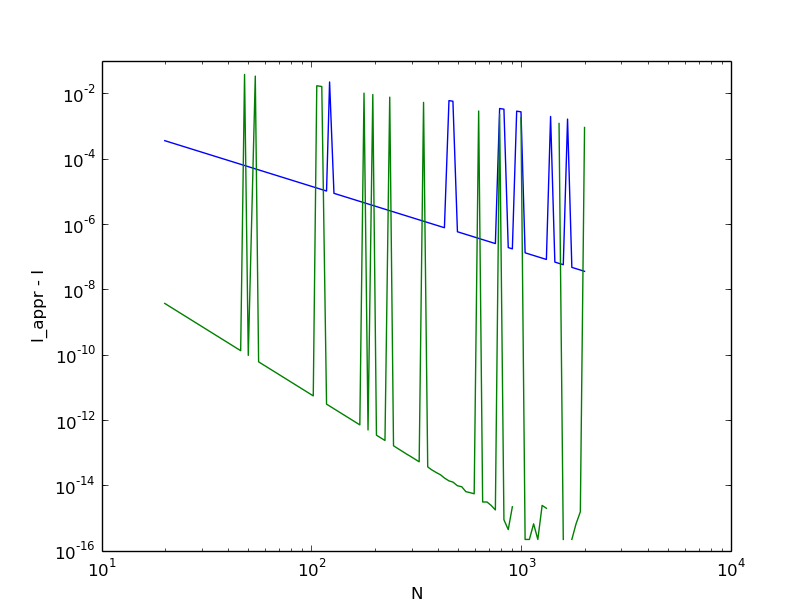
\includegraphics[width=0.5\linewidth]{fig1.png}
		\caption{Convergence rate for the trapezoidal formula (blue) and Simpson's rule (green)}
	\end{figure}
	
	The errors result due to some rounding error present while making numerical calculations with float data type. This can be remedied by using the Decimal object instead from the decimal package. Figure 2 shows the corrected convergence rate.
	
	\begin{figure}[ht!]
		\centering
		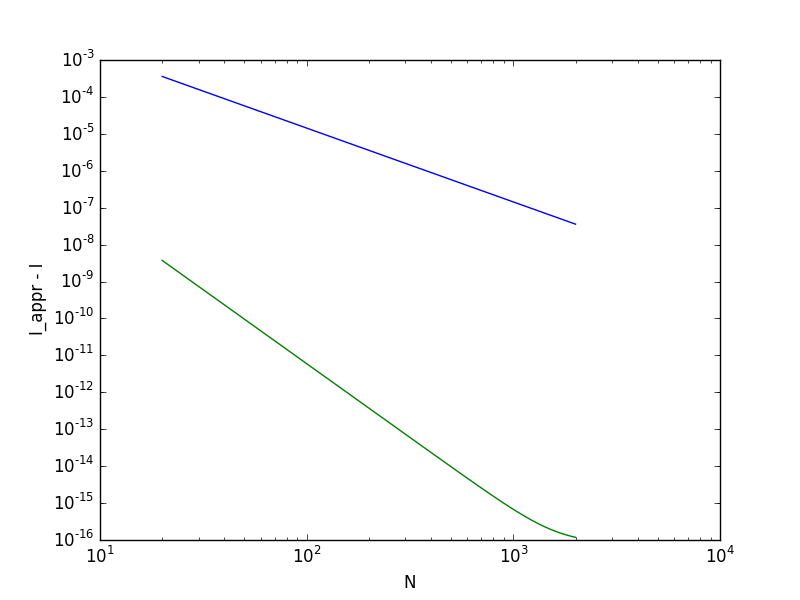
\includegraphics[width=0.5\linewidth]{fig2.png}
		\caption{Corrected Convergence rate for trapezoidal (blue) and Simpson's (green)}
	\end{figure}
	
	\item See attached code for refined Simpson's formula.
	
	The function suitably refines the extended Simpson's formula for suitable number of intervals, N, until it has a desired accuracy. It is tested on the functions $e^x$ and $x^2$ for a difference between successive approximations of less than $10^{-6}$. Table 1 shows the convergence of $e^x$ for increasing values of N. The approximation for the function $x^2$ is immediately within the desired accuracy for $N = 1$ and no further refinement is necessary.
	
	\begin{table}[!ht]
		\caption{Convergence to $e^x$}
		\begin{center}
			\begin{tabular}{| c | c | c | c |}
				\hline
				N & $I_{simp}$ & $\left|\frac{I_{simp(N)} - I_{simp(2N)}}{I_{simp(N)}}\right|$\\
				\hline \hline
				1 & 1.71886115188 & 0.000315505388119 \\ \hline
				2 & 1.71831884192 & 2.01867203012e-05 \\ \hline
				4 & 1.7182841547 & 1.26908462684e-06 \\ \hline
				8 & 1.71828197405 & 7.94340638826e-08 \\ \hline
			\end{tabular}
		\end{center}
	\end{table}
	
	\item Using \texttt{scipy.integrate.quad} and \texttt{scipy.integrate.romberg}
	
	The \texttt{scipy.integrate.quad} and \texttt{scipy.integrate.romberg} functions are able to calculate the integral much faster with a much smaller error than all of our previous functions.

\end{enumerate}



\end{document}